\section{Target Acquisition Experiment}
To understand the accuracy and performance of head-orientation-based  selection through our device, we carried out a comparative target acquisition study, where participants had to connect to wireless nodes with our technique, and a list selection approach.

\begin{figure}[t]
\centering
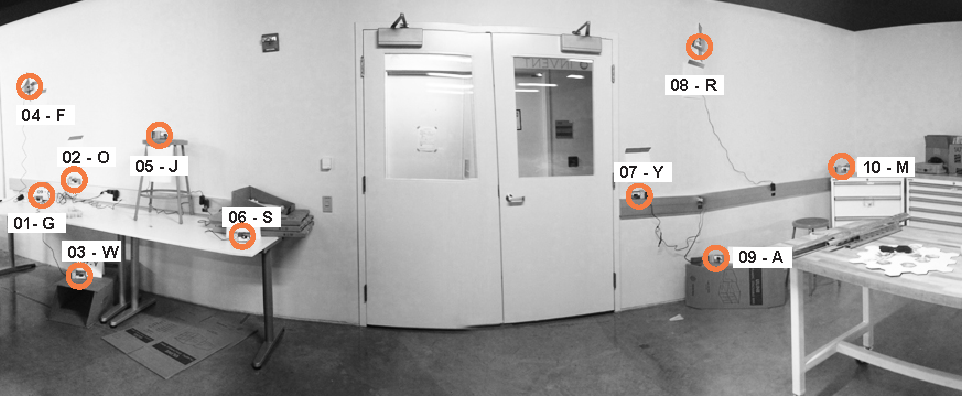
\includegraphics[width=1.0\columnwidth]{figures/targeting-study-layout.pdf}
\caption{In the targeting study, participants had to find and select one of 10 targets in a lab environment.}
\label{fig:targeting-study-layout}
\end{figure}

\subsection{Apparatus}
In an indoor environment, 10 wireless nodes are spread across a room at various heights and distances (see Figure~\ref{fig:targeting-study-layout}). The nodes are stand-ins for potential smart appliances and have all relevant functionality for targeting and selection, but do not control any actual appliances. Each node is an embedded wireless system with a microcontroller, IR receiver, a wireless XBee radio, and three status LEDs: an orange LED indicates that the device is the target that should be selected in the current trial; a red LED lights up whenever the device receives an IR signal from Glass; a blue LED shows when participants have successfully connected to a device, and is also used for disambiguation when multiple clients are within IR range (see Figure~\ref{fig:target}). Next to each client device, a paper sheet shows a number and letter combination, which are used for uniquely identifying the devices.

\begin{figure}[b]
\centering
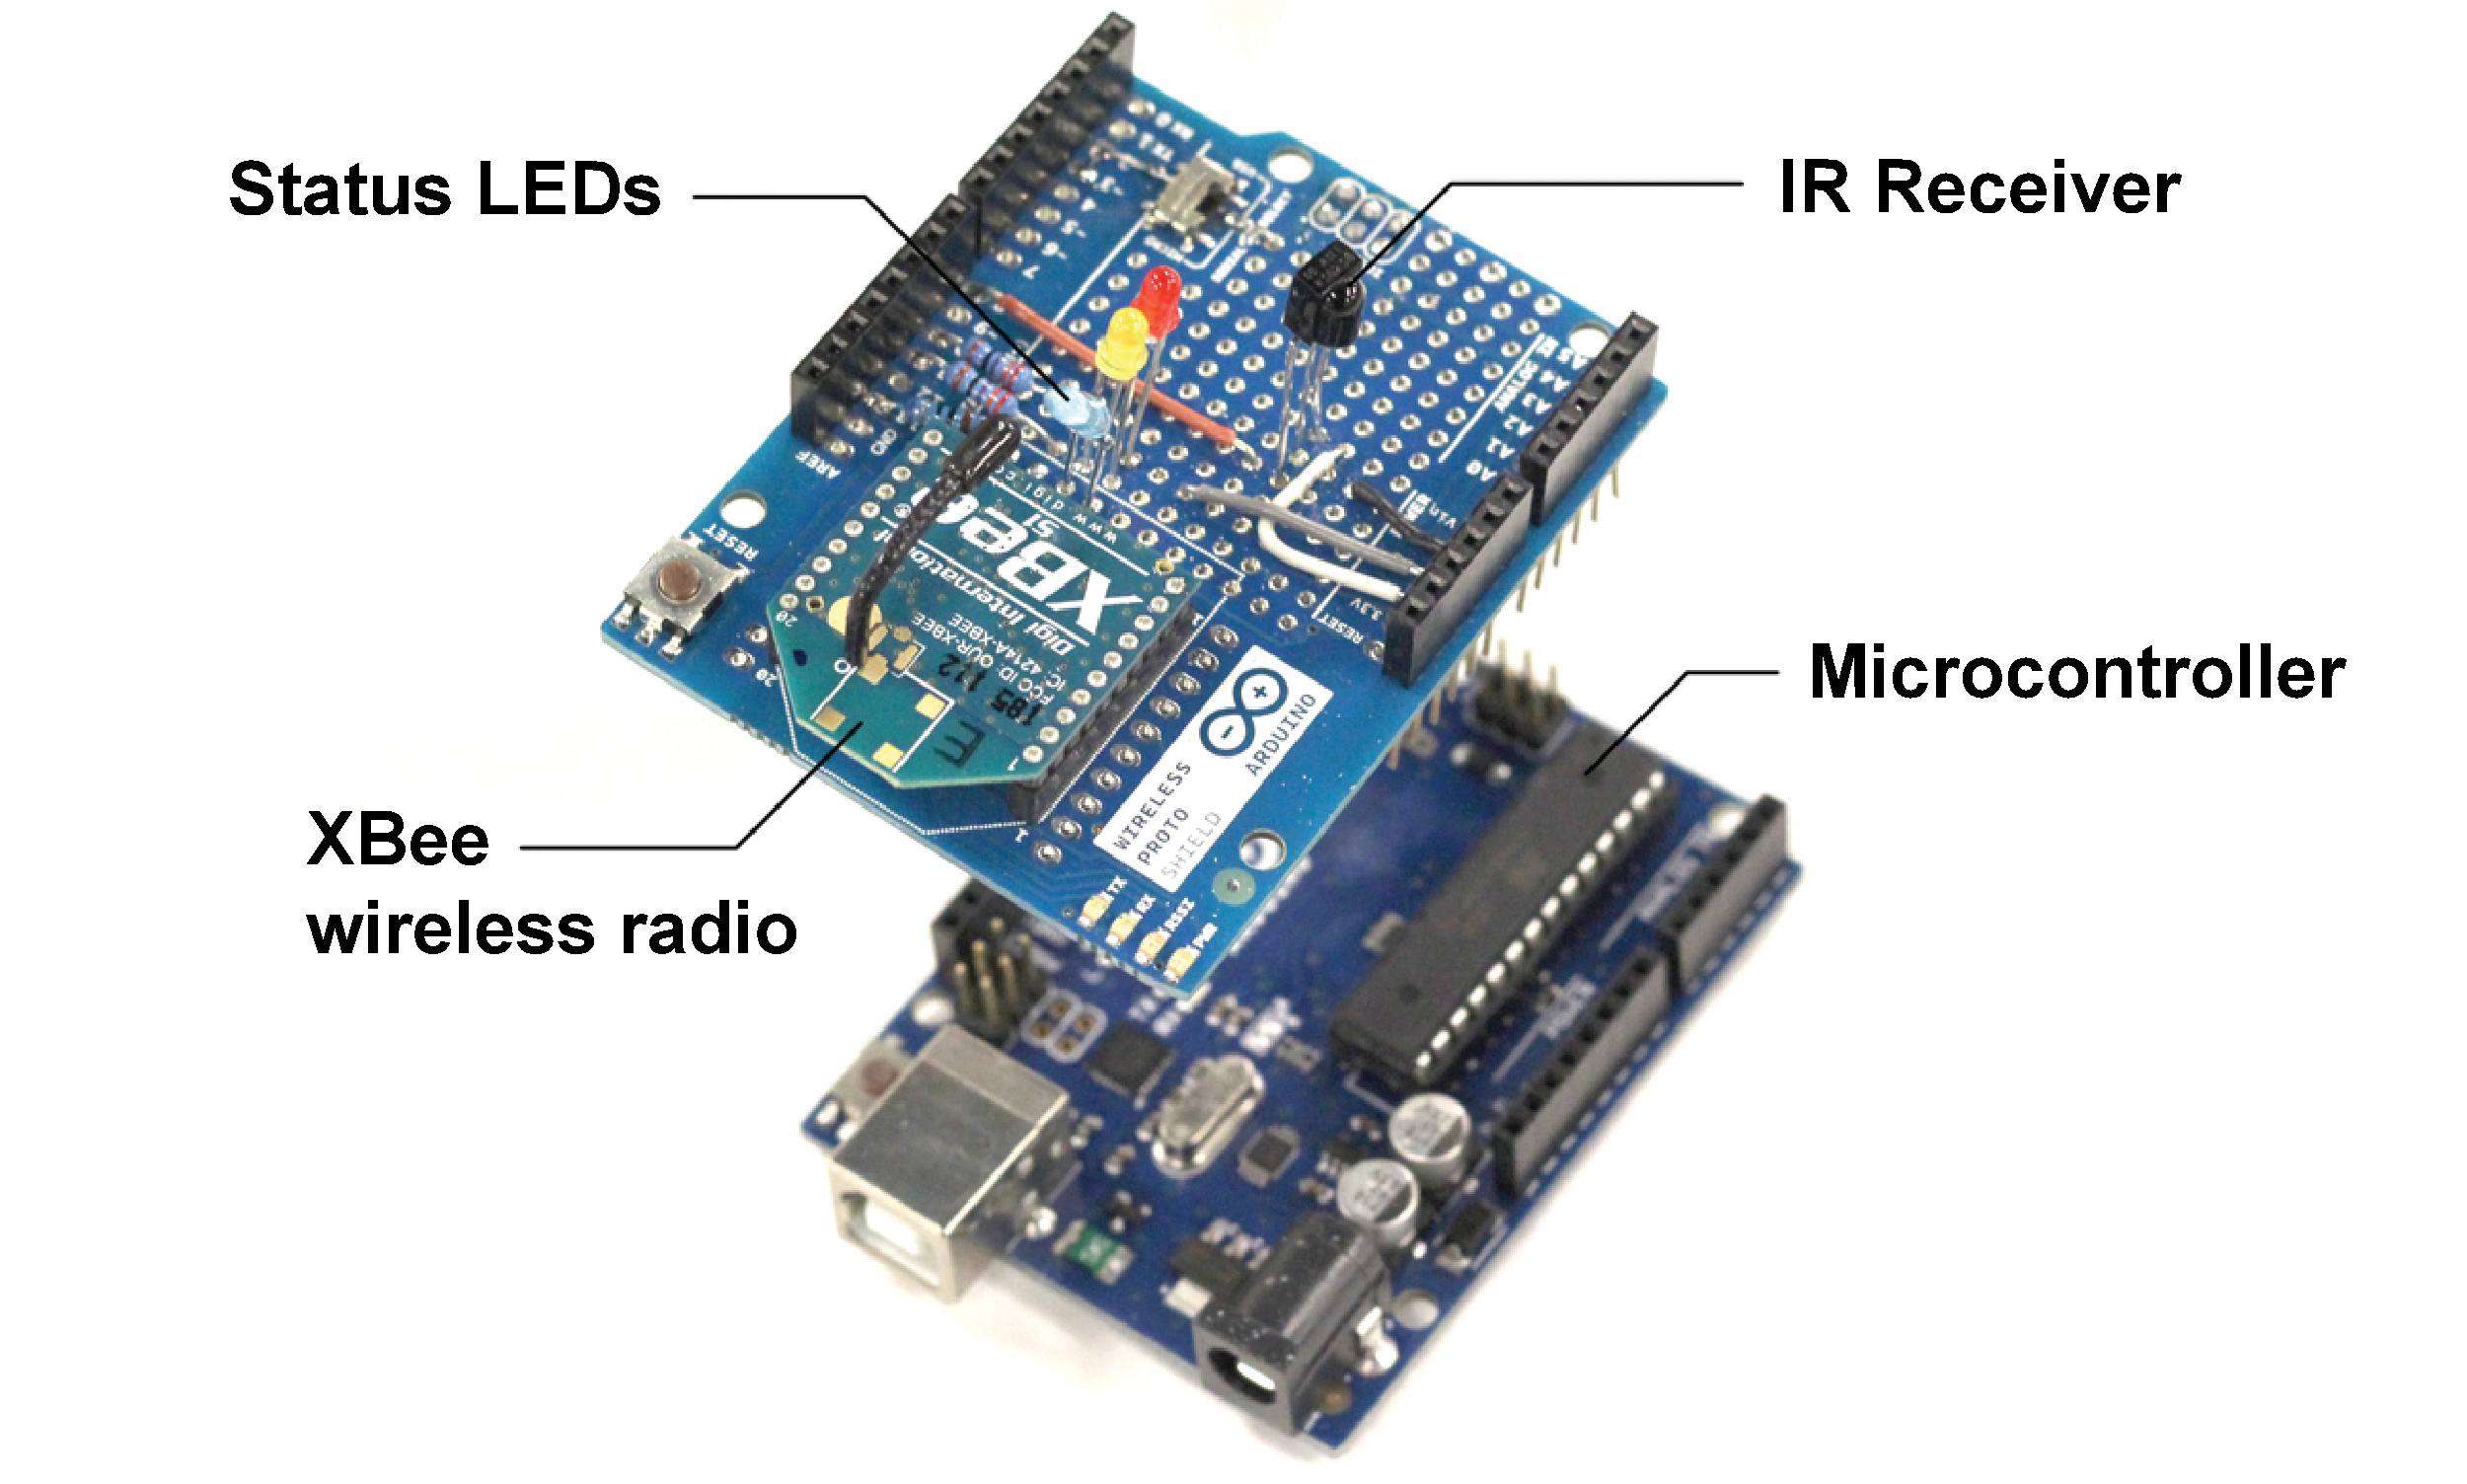
\includegraphics[width=0.8\columnwidth]{figures/study-node.pdf}
\caption{An example node from the targeting study --- we constructed 10 such nodes - each mounted in a box.}
\label{fig:targeting-study-layout}
\end{figure}

\subsection{Methodology}
In our within-subjects design, participants performed 15 target acquisition tasks each with two interaction styles. In the {\em infrared} condition, participants used our IR targeting approach; in the {\em list} condition, participants had to look up a device's letter code and select that letter code from a list displayed on their Glass device. The list was navigated with swipe motions on the Glass touchpad. For each task, participants started at a fixed position in the room. The experimenter called out a number and simultaneously started a timer. Participants then had to find the number on sheets printed and affixed to walls and other surfaces. In the {\em infrared} condition, participants then selected and acquired the target by aiming the infrared beam at the target, and confirmed their selection with a touchpad tap. If more than one target was within range, participants had to either use the disambiguation dialog or reposition themselves. In the {\em list} condition, participants had to read the letter next to the number and then select that letter by browsing a linear list shown in their Glass display. While the list was alphabetized, letter arrangement in the room was not. This design required participants to find the target in the room before starting a list navigation to keep conditions similar to each other.

Afterwards, participants completed a survey that elicited answers to Likert-scale questions as well as open-ended answers about their experience.

\subsection{Participants}
We recruited N participants from our institution. X had never used Glass before.

\subsection{Measures}
The main measure was {\bf target acquisition time}: the time required to identify, select, and connect to a wireless target device. We also elicited {\bf user preference}: which interface users preferred for the task after completing the study.

\subsection{Results}

\subsubsection{Performance data}

\subsubsection{User preference}
X of Y users preferred infrared mode over list mode. As slef-report data can skew to please experimenters, we also asked participants to elucidate why they preferred one interface over the other.

\bjoern{Insert summary of survey data on this point here.}

\subsubsection{Qualitative results}

